The Tag-and-Probe study was performed on the EGM dataset using the golden JSON of ~58.83 fb$^{-1}$. More details on the Tag-and-Probe method can be found in Ref.~\cite{AN-15-277}. 

Tag electrons need to satisfy the following quality requirements:
\begin{itemize}
%\item trigger matched to HLT\_Ele27\_eta2p1\_WPTight\_Gsf\_v*
\item~trigger matched to single electron trigger (e.g HLT\_Ele32\_WPTight\_Gsf\_L1DoubleEG\_v* for 2018 for instance)
\item~$p_{T} > 30$~GeV (tag), super cluster (SC) $\eta < 2.17$% but on in EB-EE gap ($1.4442<|\eta|<1.566$)
\item~the tag and the probe need to have opposite charge.
%\item tight working point of the Spring16 cut-based electron ID
\end{itemize}

For the bin between 7 and 20 GeV, additional criteria are required: 
\begin{itemize}
\item~the tag has to pass a cut on the MVA ID$>0.92$, $\sqrt(2*PFMET*p_T(tag)*(1-cos(\phi_{MET}-\phi_{tag})))<45 GeV$.
\item~tag $p_{T}$ increased to 50 GeV
\item~the charge is determined with the so-called selection method, asing all three estimates of the electron charge to agree.
\end{itemize}
%t
These additional requirements help cleaning the background and makes the fits more reliable (and thus, the measurement more precise).

Probe electrons only need to be reconstructed as GsfElectron while the FSR recovery algorithm is not applied in efficiency measurement. 

The nominal MC efficiencies are evaluated from the LO MadGraph Drell-Yan, while the NLO systematics use the MadGraph\_AMCatNLO sample (or POWHEG in 2018).

For the efficiency measurements a template fit is used. The $m_{ee}$ signal shape of the passing and failing probes is taken from MC and convoluted with a Gaussian. The data is then fitted with the convoluted MC template and a CMSShape (an Error-function with a one-sided exponential tail). This change follows from the usage of the T\&P tool developed by the EGM POG. For the low $p_T$ bins, a gaussian is added to the signal model for the failing probes. 

%\paragraph{Electron selection efficiency measurements}\mbox{}\\
%\label{par:Efficiency_measurements}

The electron selection efficiency is measured as a function of the probe electron $p_{T}$ and its SC $\eta$, and separately for electrons falling in the ECAL gaps. Figure \ref{fig:ele_sel_pt_turn_onA},~\ref{fig:ele_sel_pt_turn_onB},~\ref{fig:ele_sel_pt_turn_onC} and~\ref{fig:ele_sel_eta_turn_onA},\ref{fig:ele_sel_eta_turn_onB},~\ref{fig:ele_sel_eta_turn_onC} show the $p_{T}$ and $\eta$ turn-on curves measured in data, for 2016, 2017 and 2018.
% and the final 2D scale factor is shown in Fig.~\ref{fig:ele_sel_scale_factors} together with the systematic uncertainties. %These scale factors are very similar to the ICHEP figures, but more homogenous across $\eta$ and $p_{T}$ because of the higher statistics and the usage of more stable fitting routines in the new T\&P tool.

%\includegraphics[page=2, width=0.4\textwidth]{Figures/Electrons/ErecoEta}\\

\begin{figure}[!htb]
\begin{center}
    \subfigure [] {\resizebox{7.5cm}{!}{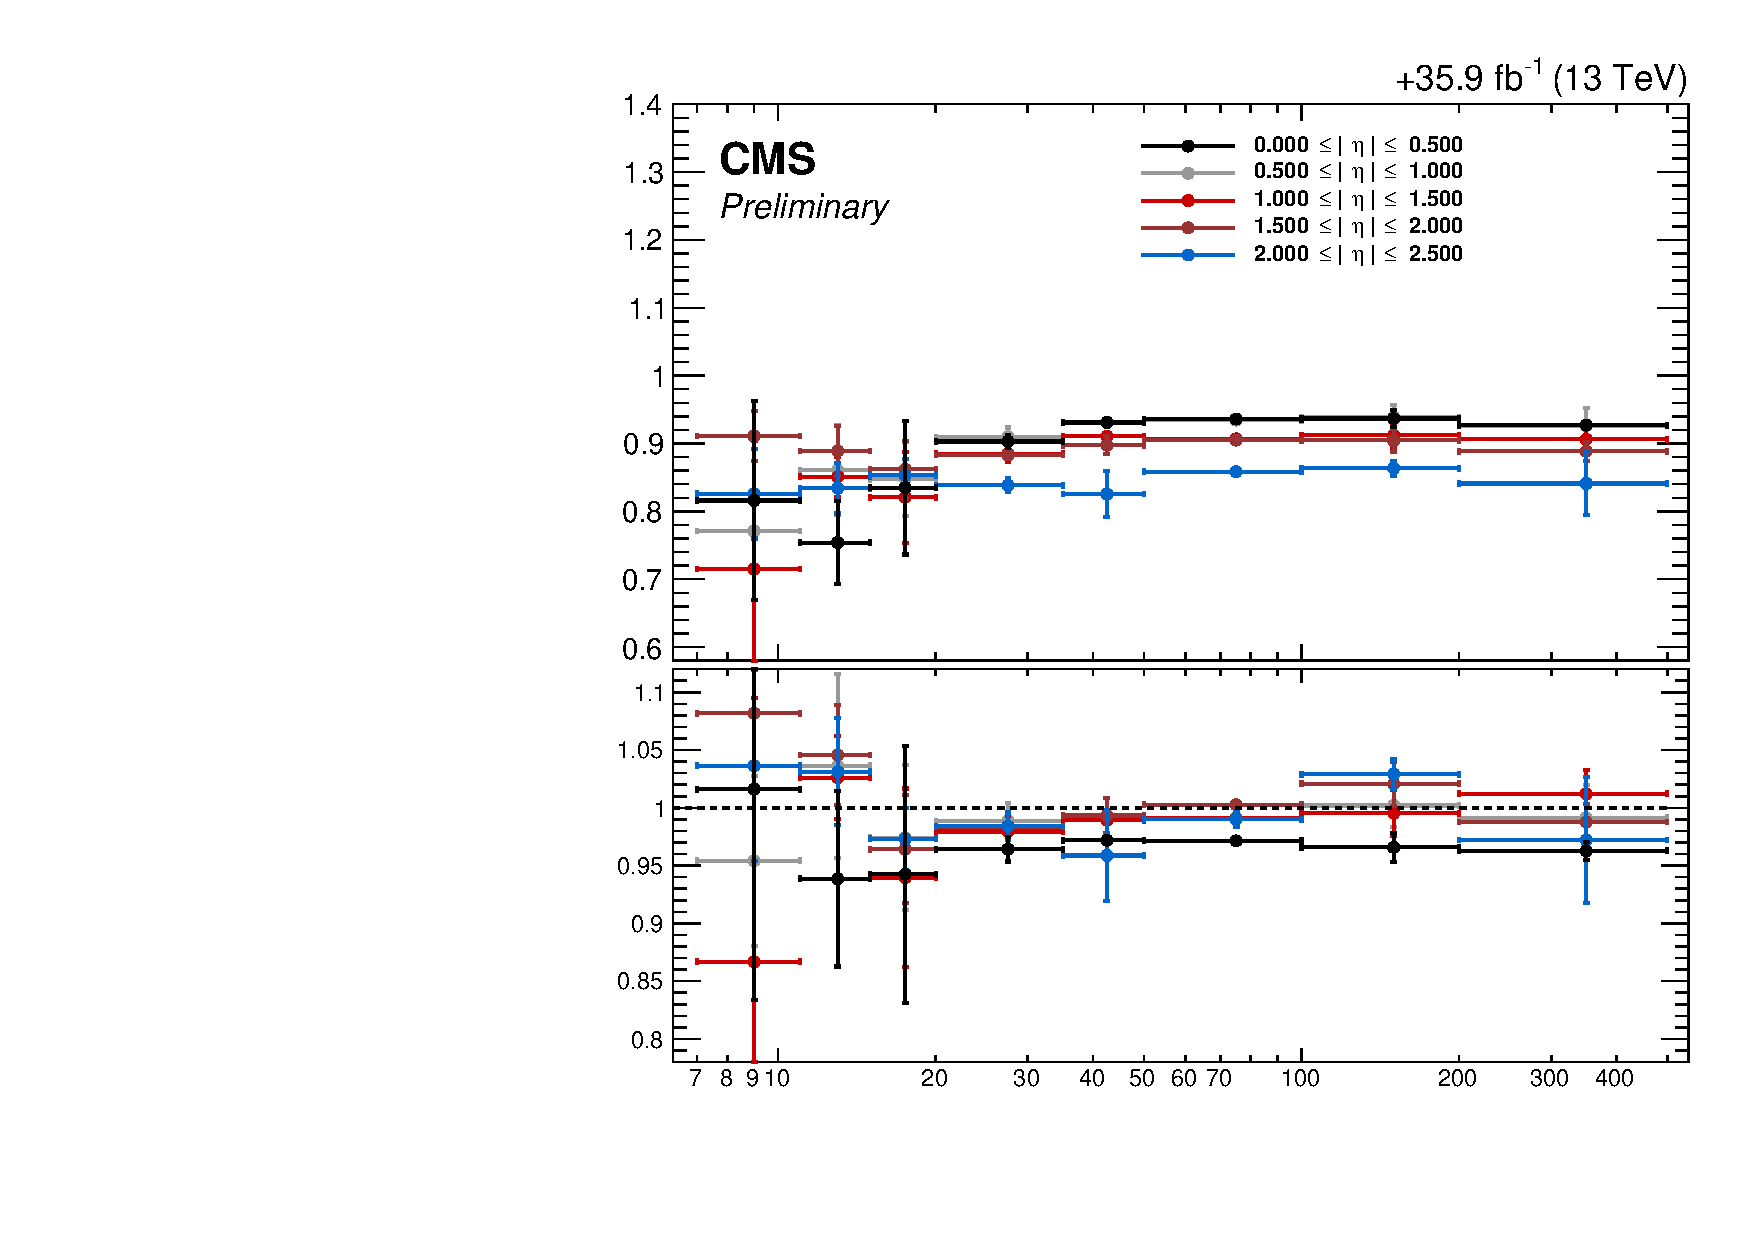
\includegraphics[page=1]{Figures/Electrons/2016_egammaEffitxt_egammaPlots.pdf}}} %eleSFvspT.png}}}
    \subfigure [] {\resizebox{7.5cm}{!}{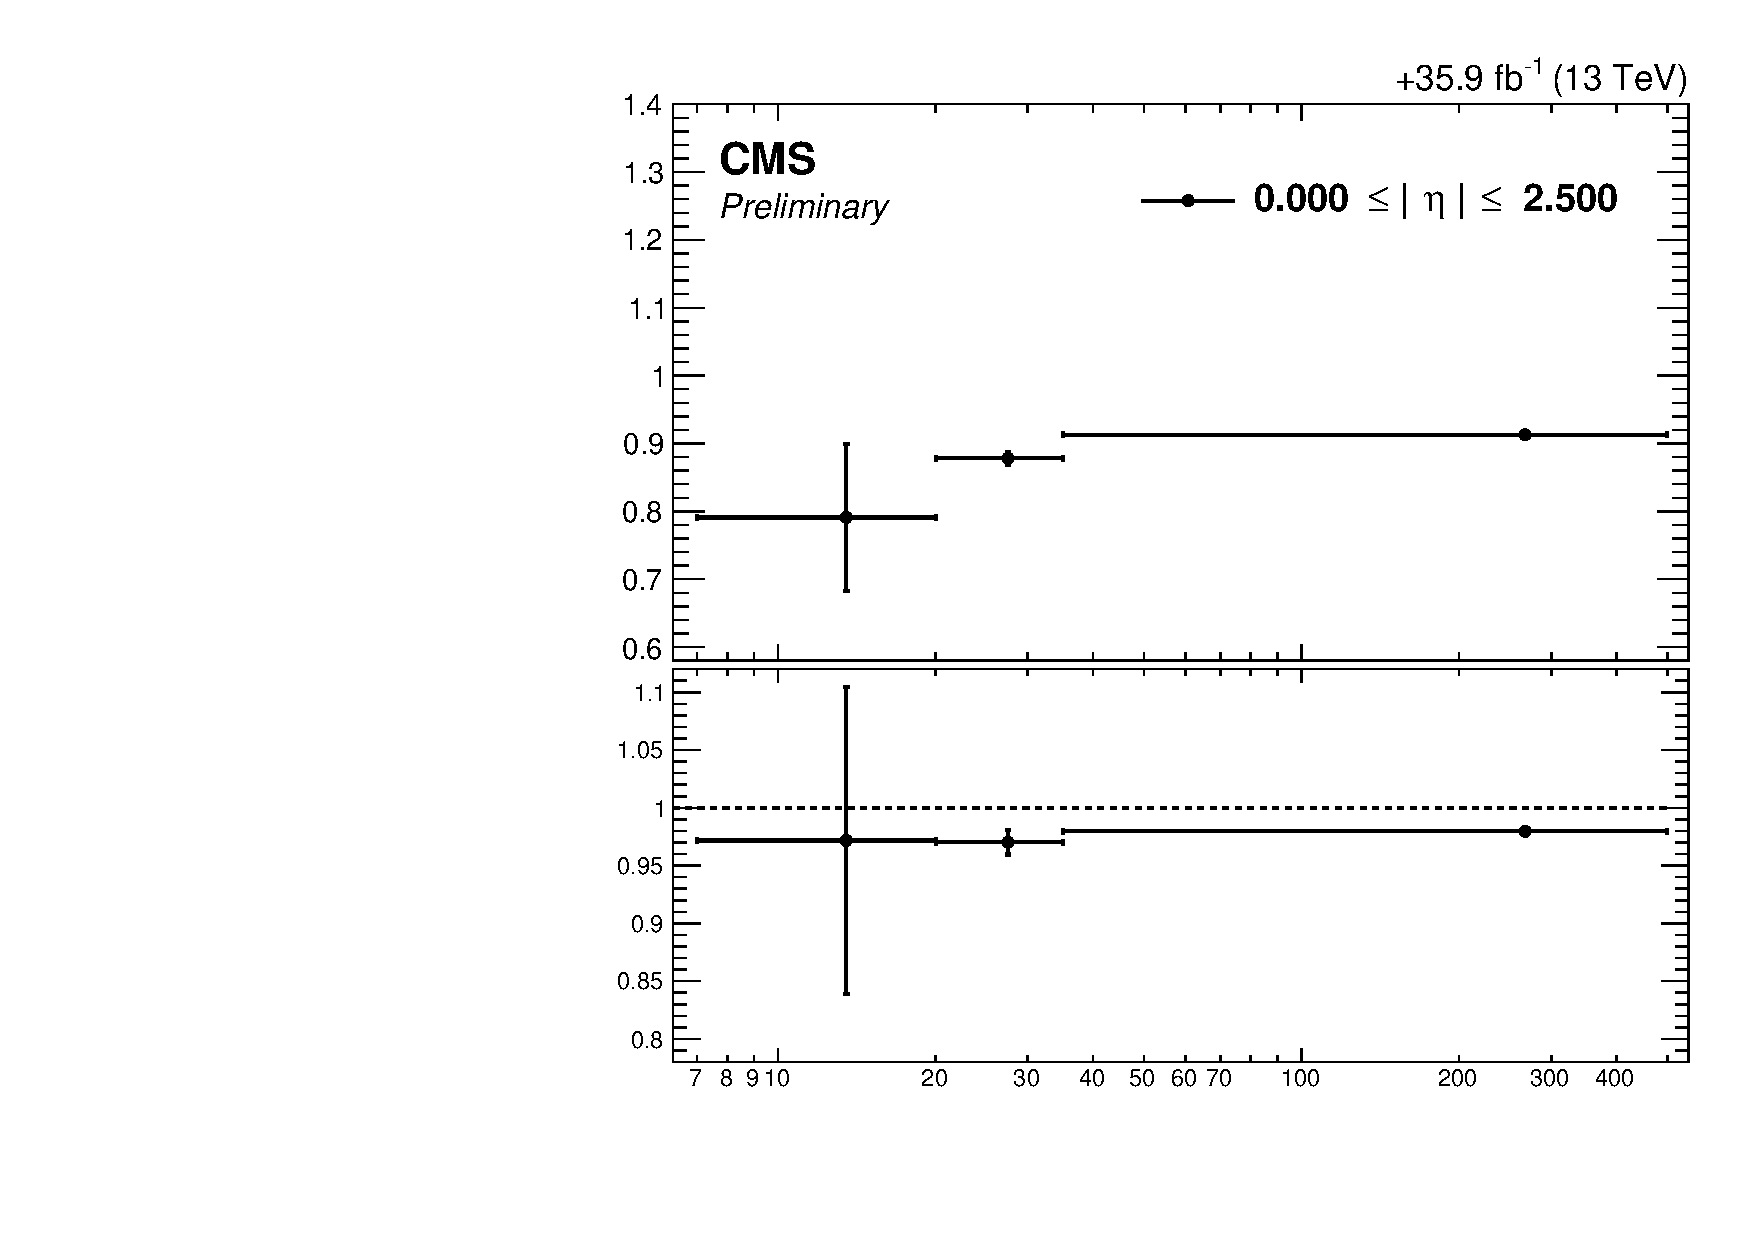
\includegraphics[page=1]{Figures/Electrons/2016_egammaEffitxt_egammaPlotsGAP.pdf}}} \\
    %    \subfigure [] {\resizebox{7.5cm}{!}{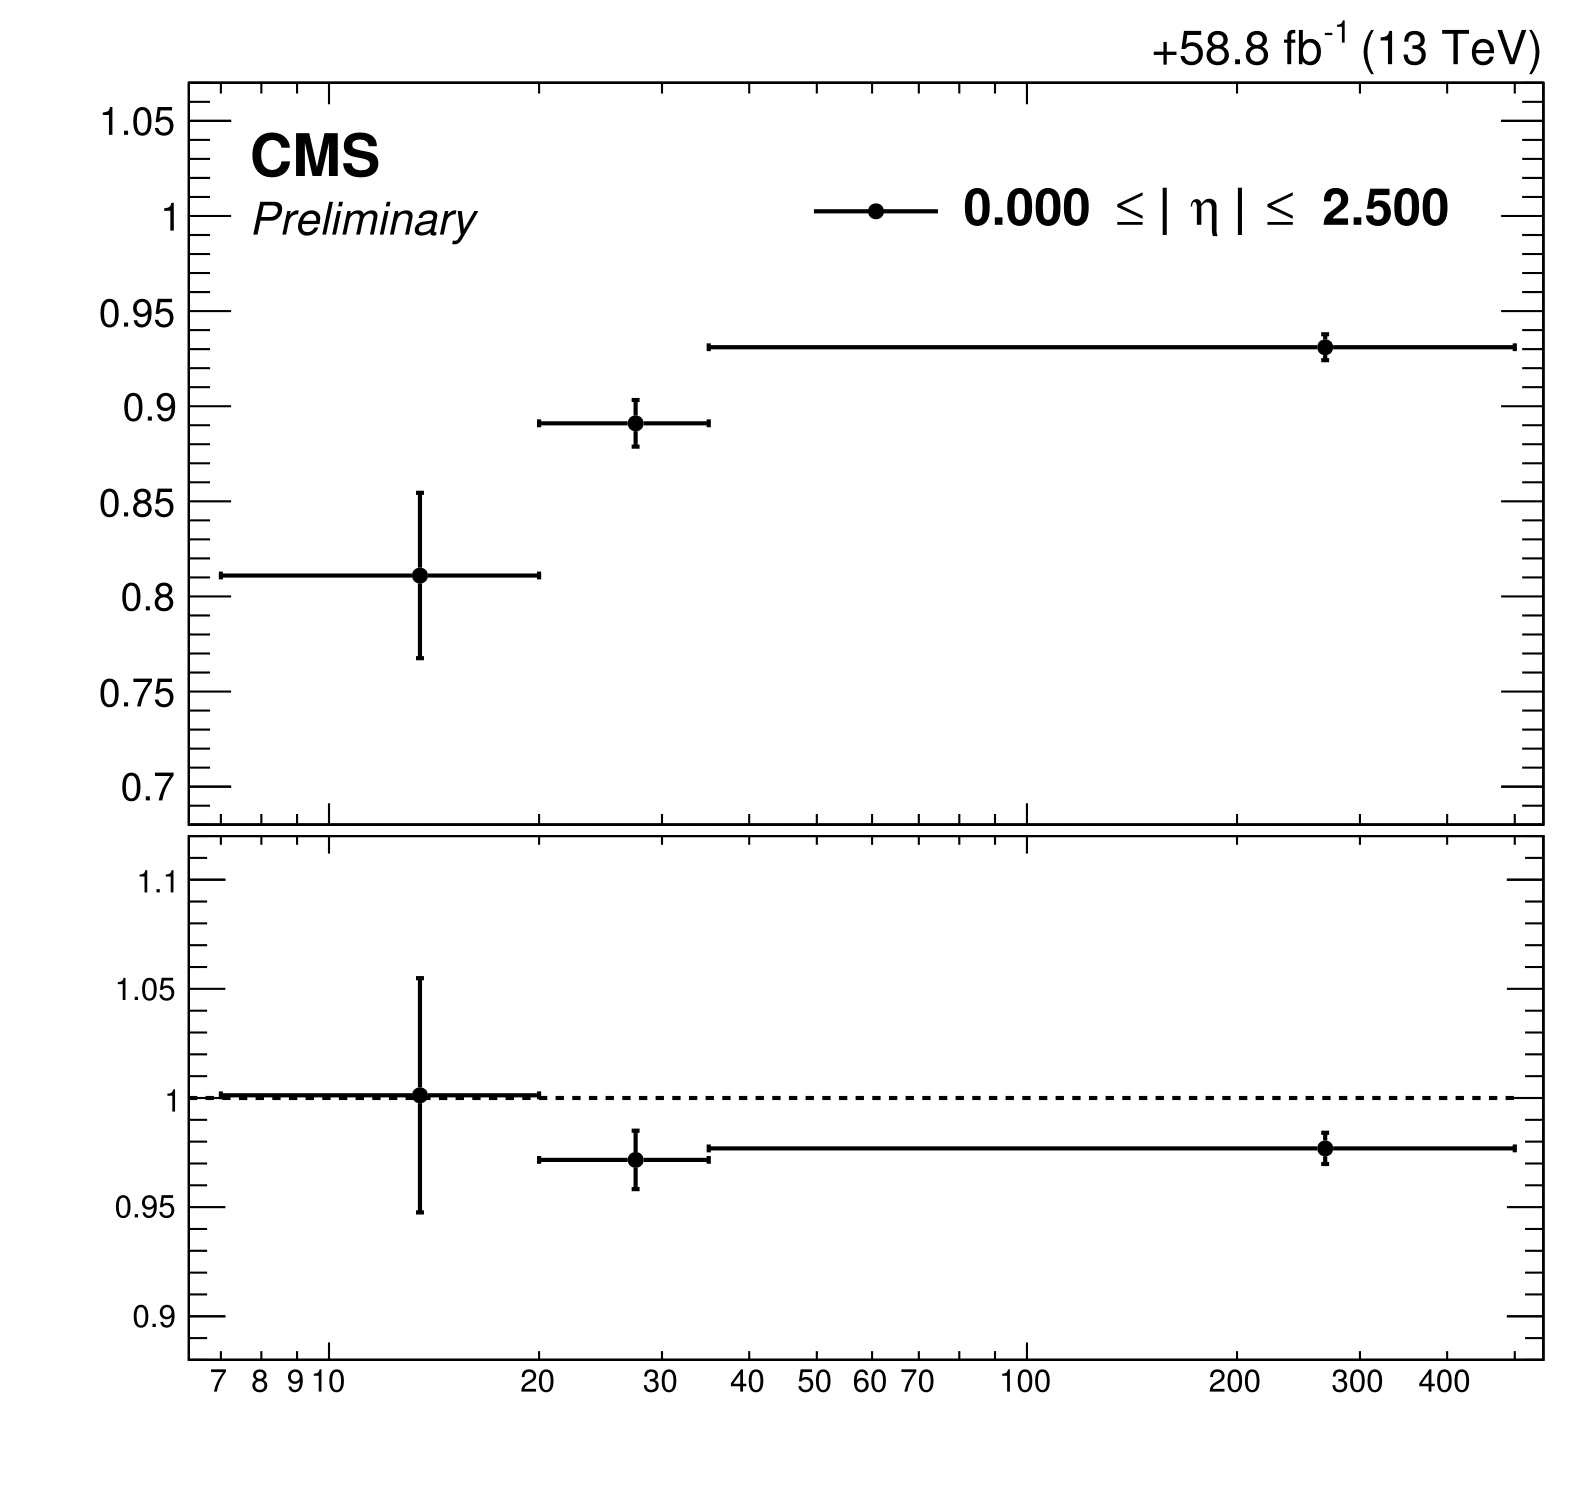
\includegraphics{Figures/Electrons/eleSFvspTgap.png}}}\\
\caption{Electron selection efficiencies vs $p_T$ measured using the Tag-and-Probe technique described in the text, non-gap electrons (left) and gap electrons (right), together with the corresponding data/MC ratio (bottom), for 2016 samples.}
\label{fig:ele_sel_pt_turn_onA}
\end{center}
\end{figure}

\begin{figure}[!htb]
\begin{center}
    \subfigure [] {\resizebox{7.5cm}{!}{\includegraphics[page=2]{Figures/Electrons/2016_egammaEffitxt_egammaPlots.pdf}}}
    \subfigure [] {\resizebox{7.5cm}{!}{\includegraphics[page=2]{Figures/Electrons/2016_egammaEffitxt_egammaPlotsGAP.pdf}}}\\
\caption{Electron selection efficiencies vs $\eta$ measured using the Tag-and-Probe technique described in the text, non-gap electrons (left) and gap electrons (right), together wit the corresponding data/MC ratio at the bottom of each plot, for 2016 samples. Dashed lines is MC, solid lines is DATA.}
\label{fig:ele_sel_eta_turn_onA}
\end{center}
\end{figure}

\begin{figure}[!htb]
\begin{center}
    \subfigure [] {\resizebox{7.5cm}{!}{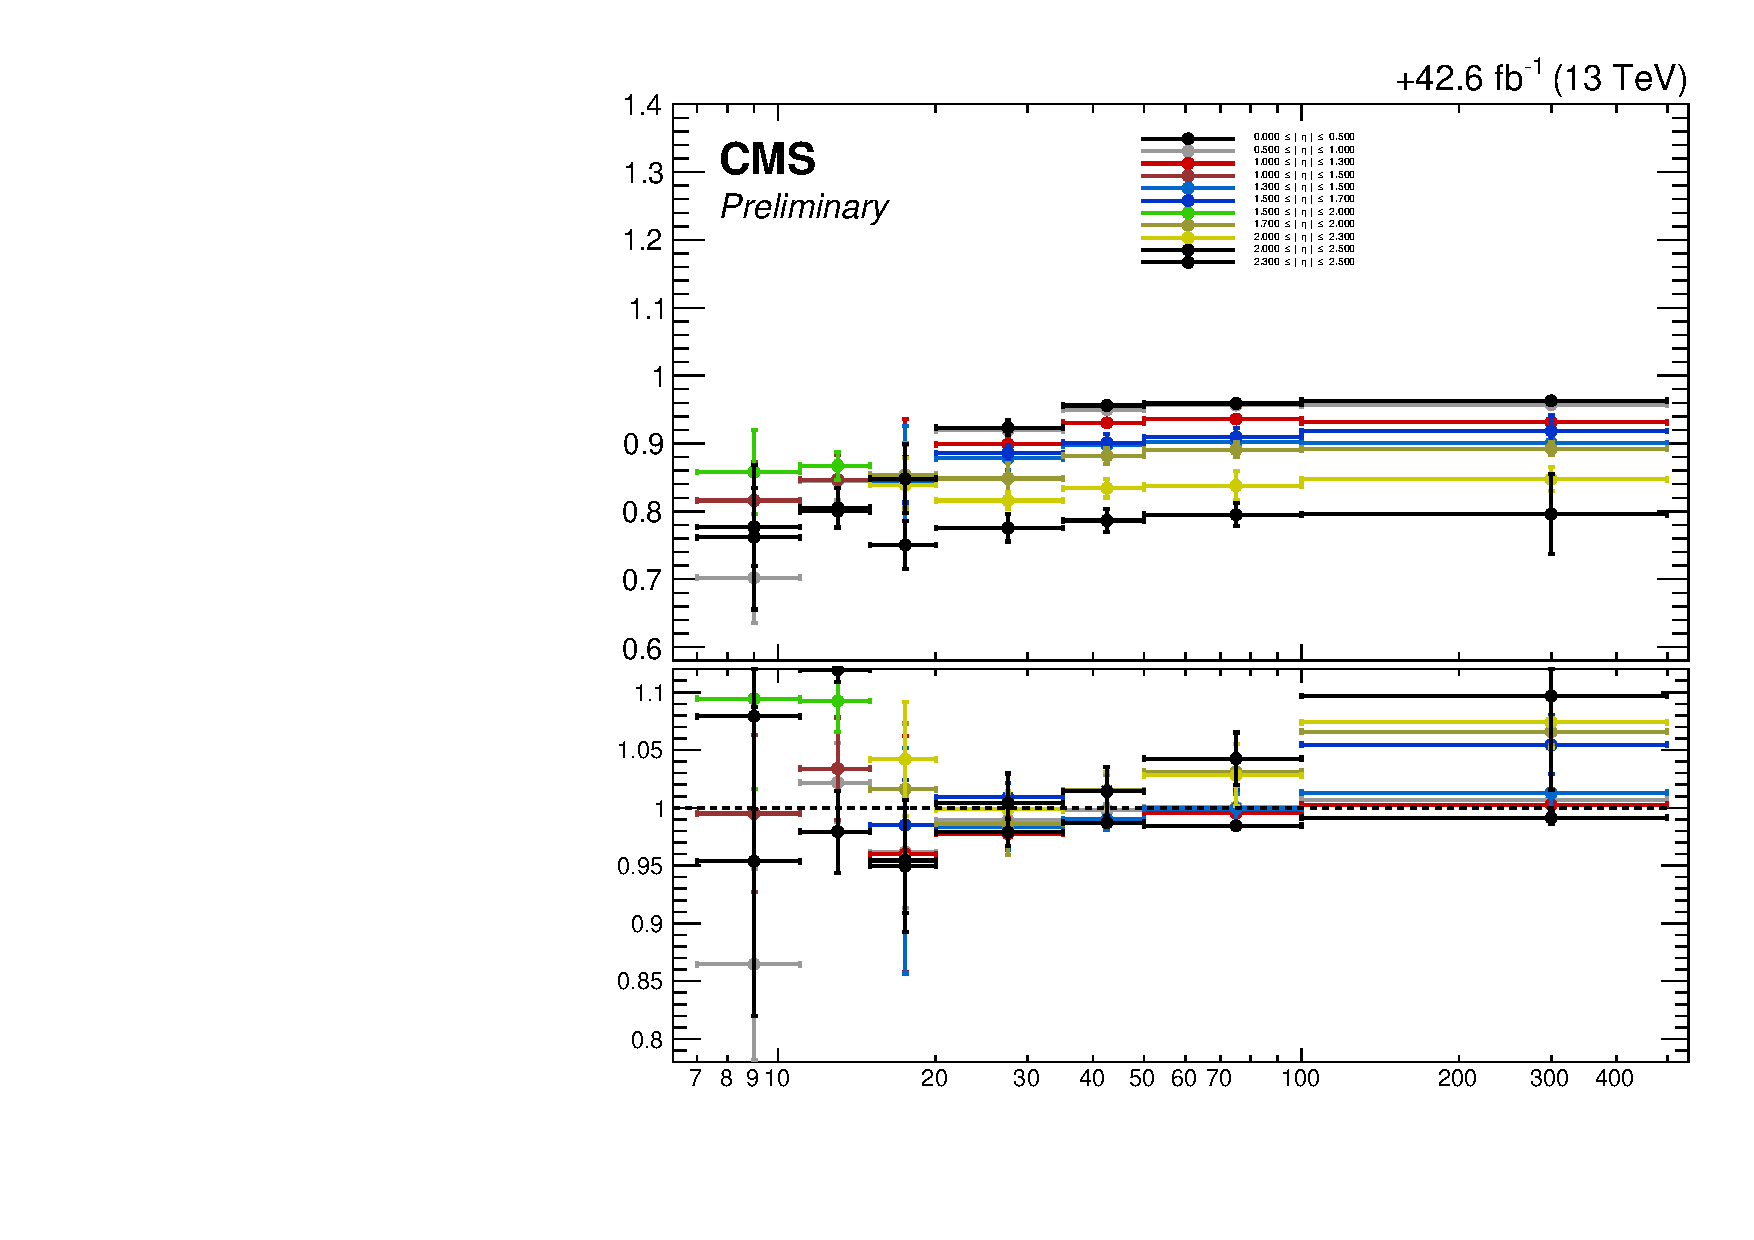
\includegraphics[page=1]{Figures/Electrons/2017_egammaEffitxt_egammaPlots.pdf}}} %eleSFvspT.png}}}
    \subfigure [] {\resizebox{7.5cm}{!}{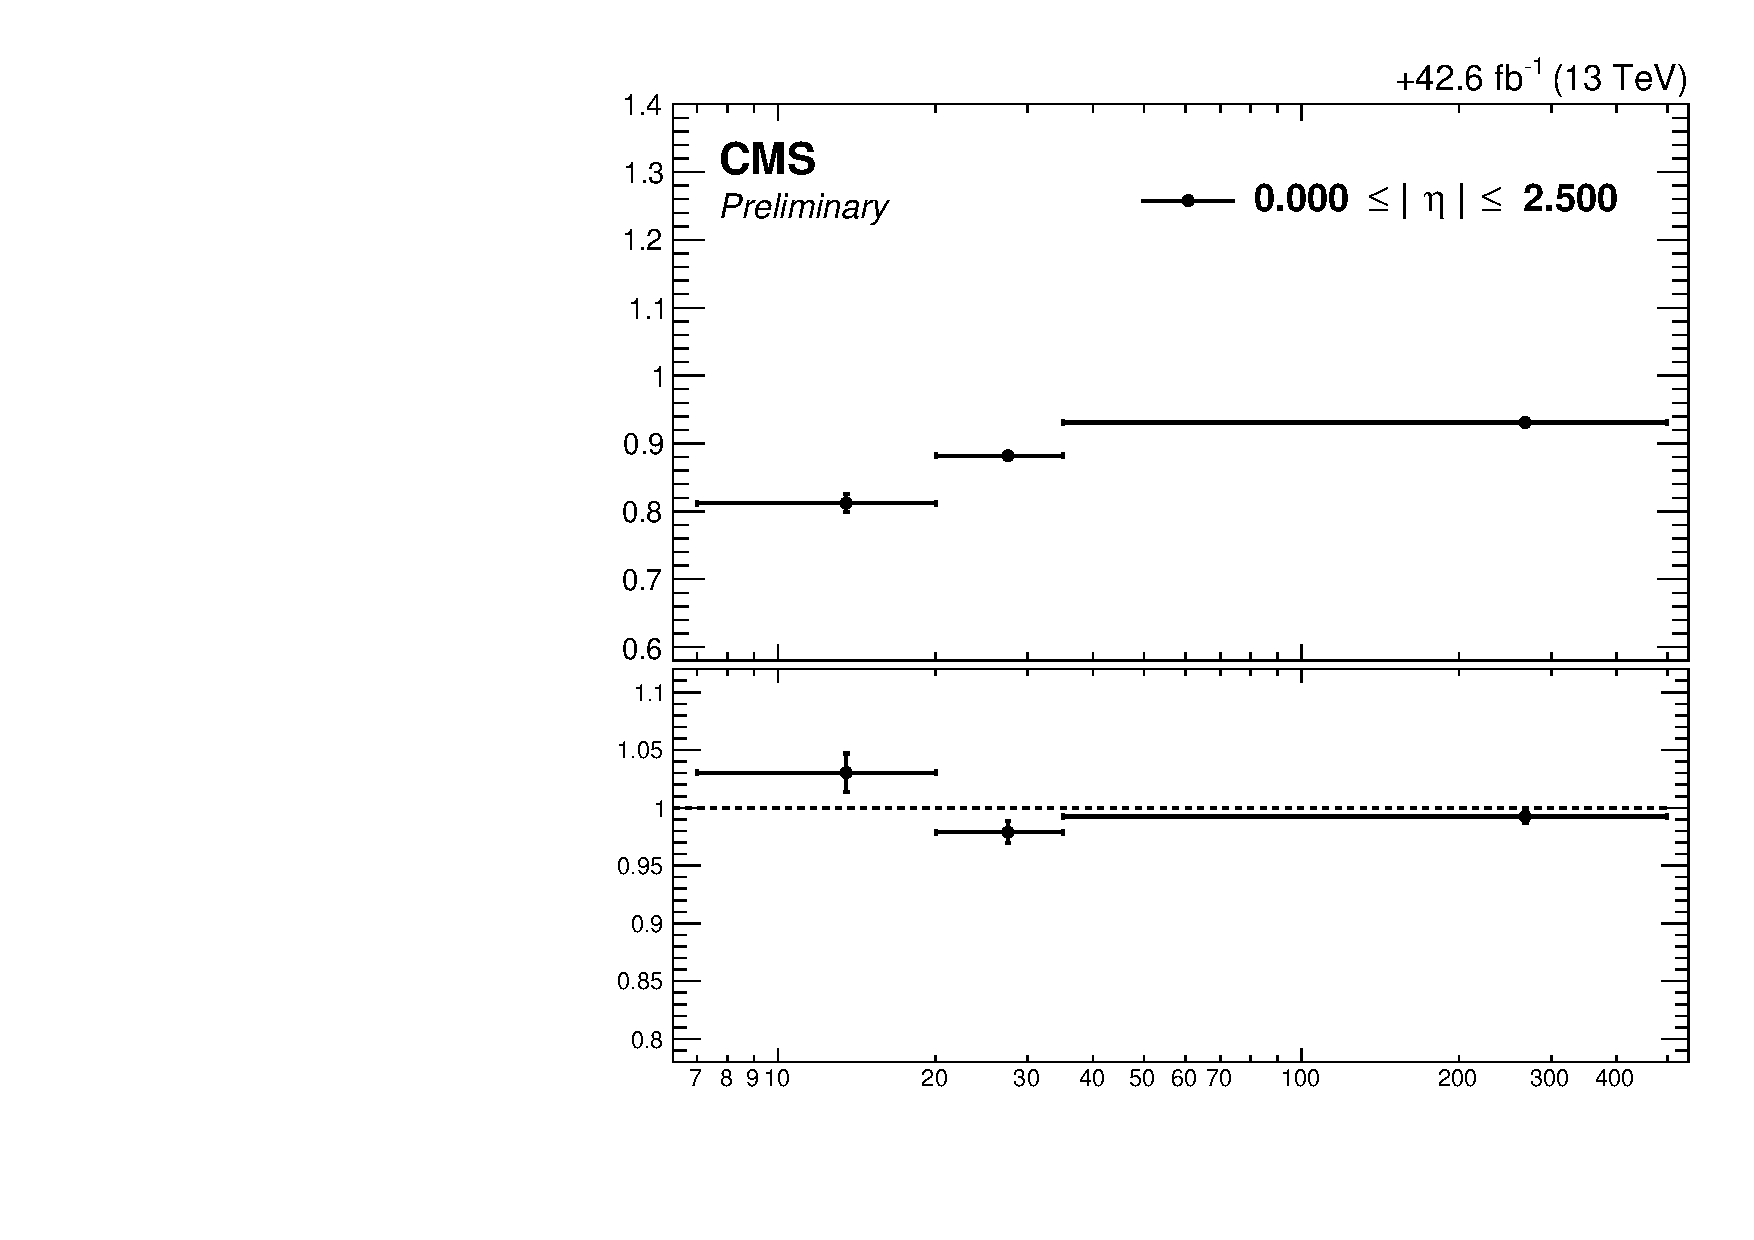
\includegraphics[page=1]{Figures/Electrons/2017_egammaEffitxt_egammaPlotsGAP.pdf}}} \\
    %    \subfigure [] {\resizebox{7.5cm}{!}{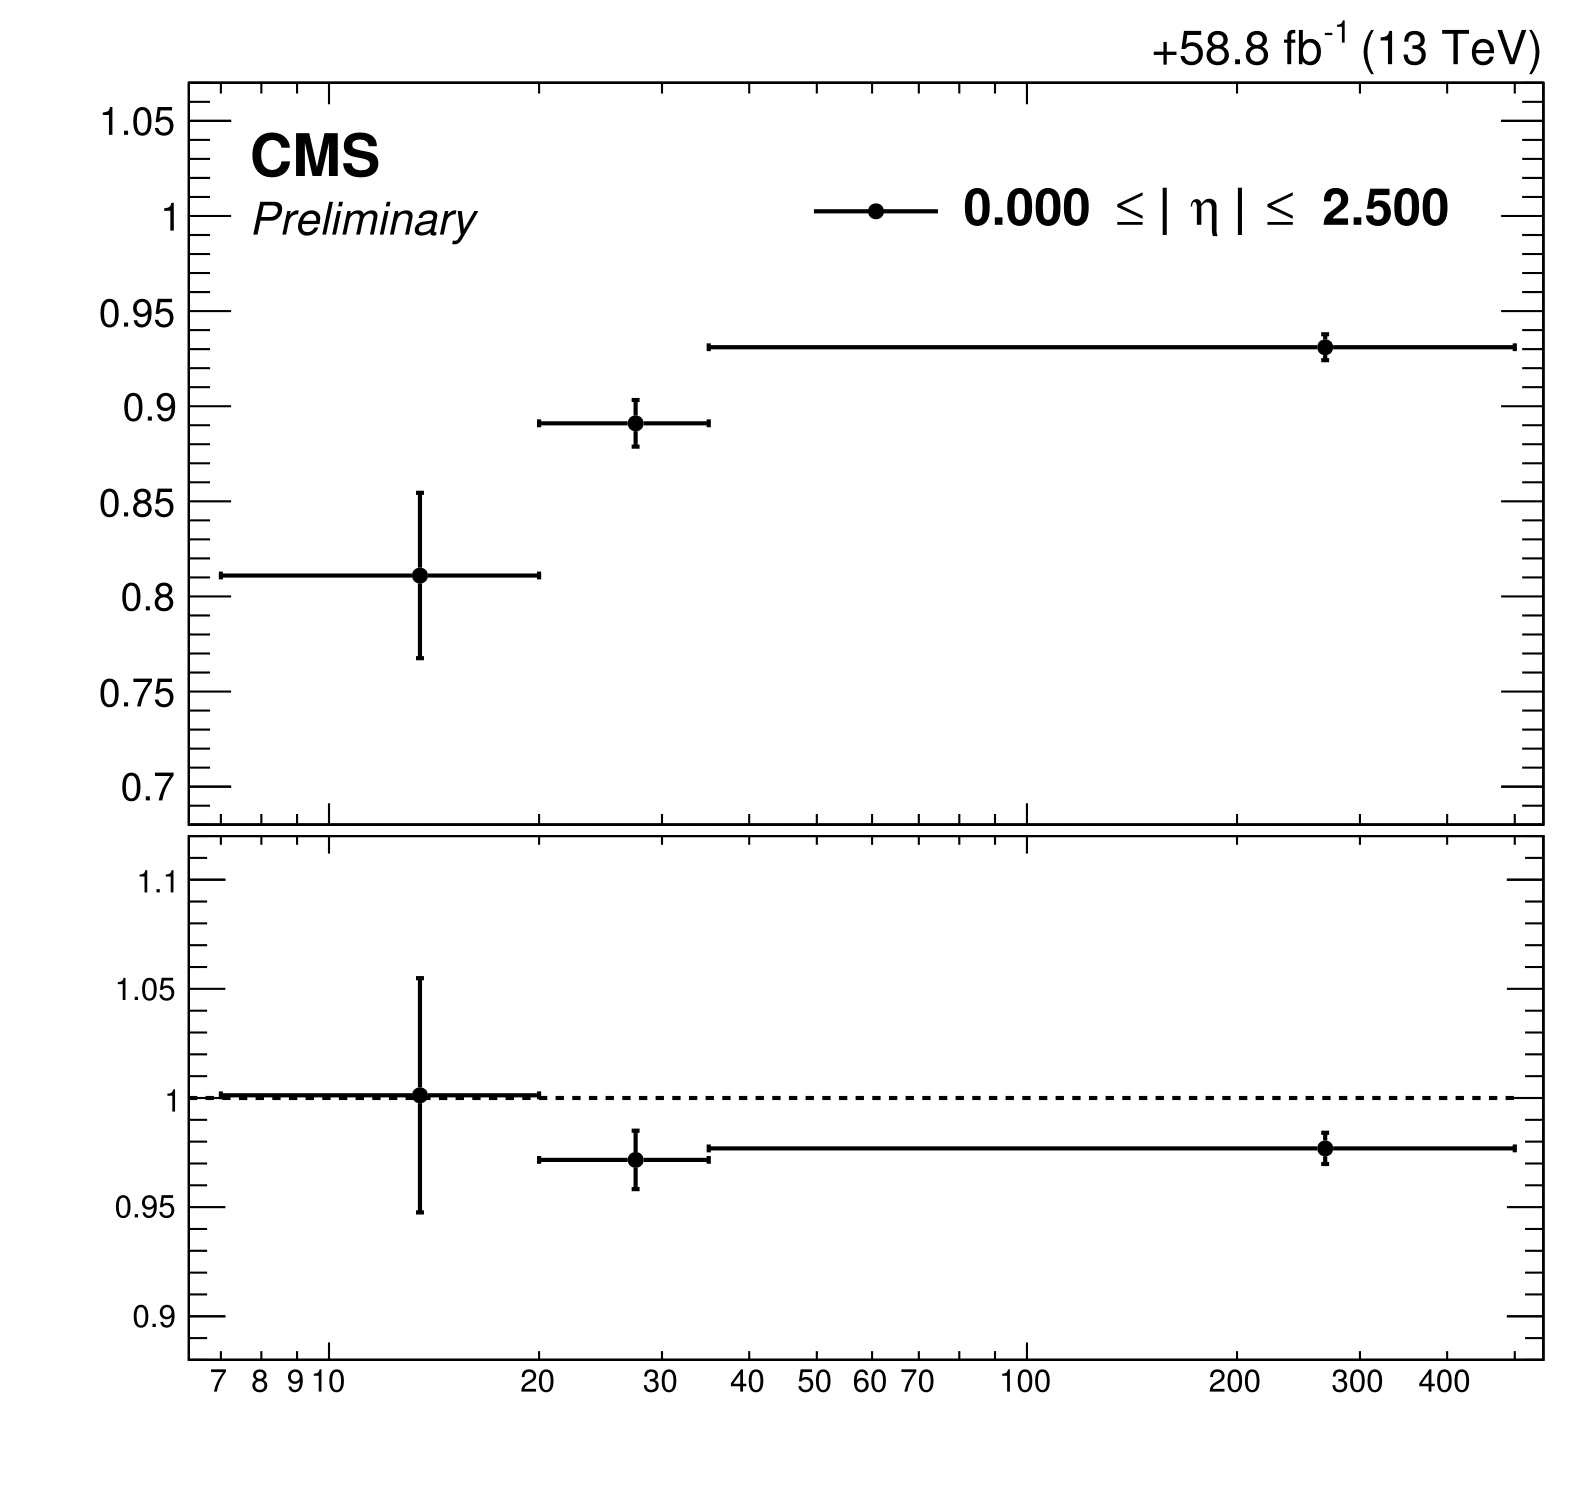
\includegraphics{Figures/Electrons/eleSFvspTgap.png}}}\\
\caption{Electron selection efficiencies vs $p_T$ measured using the Tag-and-Probe technique described in the text, non-gap electrons (left) and gap electrons (right), together with the corresponding data/MC ratio (bottom), for 2017 samples.}
\label{fig:ele_sel_pt_turn_onB}
\end{center}
\end{figure}

\begin{figure}[!htb]
\begin{center}
    \subfigure [] {\resizebox{7.5cm}{!}{\includegraphics[page=2]{Figures/Electrons/2017_egammaEffitxt_egammaPlots.pdf}}}
    \subfigure [] {\resizebox{7.5cm}{!}{\includegraphics[page=2]{Figures/Electrons/2017_egammaEffitxt_egammaPlotsGAP.pdf}}}\\
\caption{Electron selection efficiencies vs $\eta$ measured using the Tag-and-Probe technique described in the text, non-gap electrons (left) and gap electrons (right), together wit the corresponding data/MC ratio at the bottom of each plot, for 2017 samples. Dashed lines is MC, solid lines is DATA.}
\label{fig:ele_sel_eta_turn_onB}
\end{center}
\end{figure}

\begin{figure}[!htb]
\begin{center}
    \subfigure [] {\resizebox{7.5cm}{!}{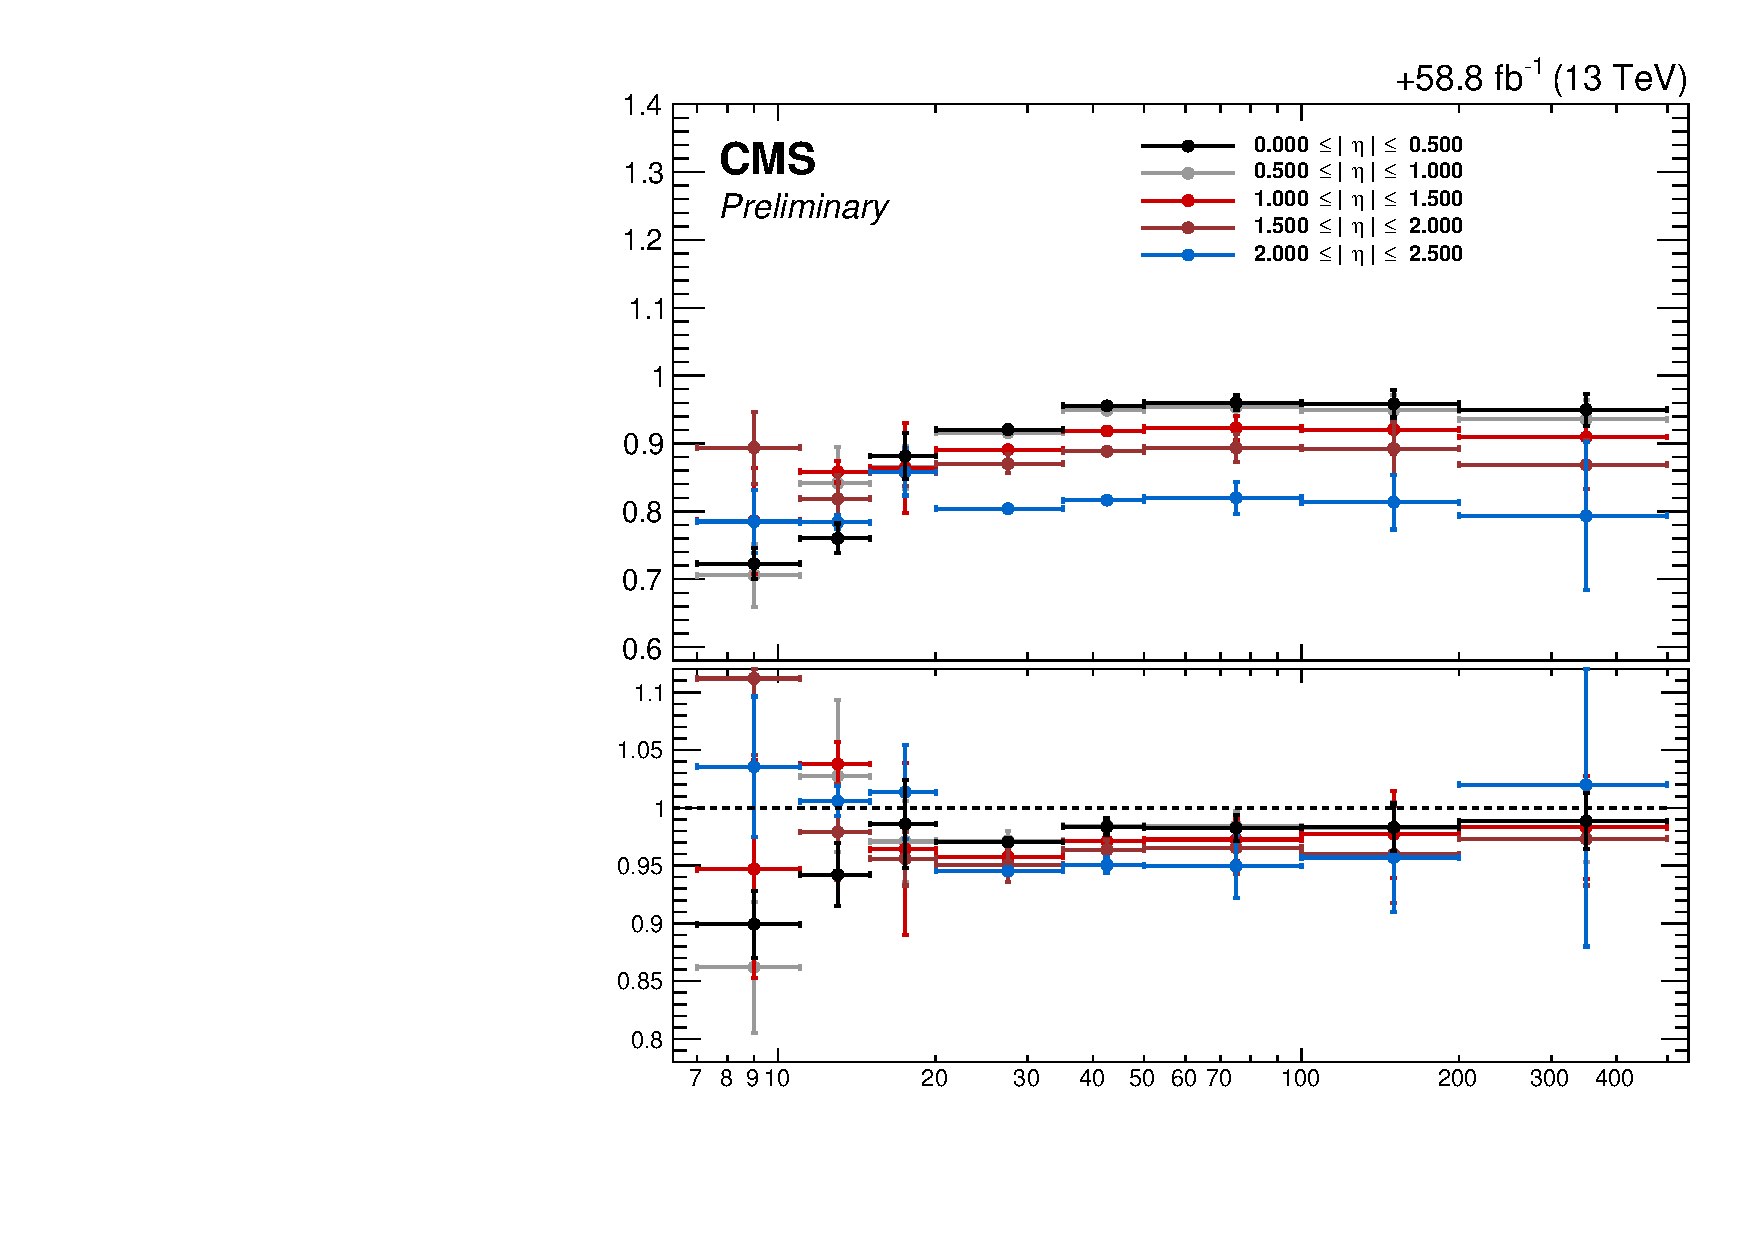
\includegraphics[page=1]{Figures/Electrons/2018_egammaEffitxt_egammaPlots.pdf}}} %eleSFvspT.png}}}
    \subfigure [] {\resizebox{7.5cm}{!}{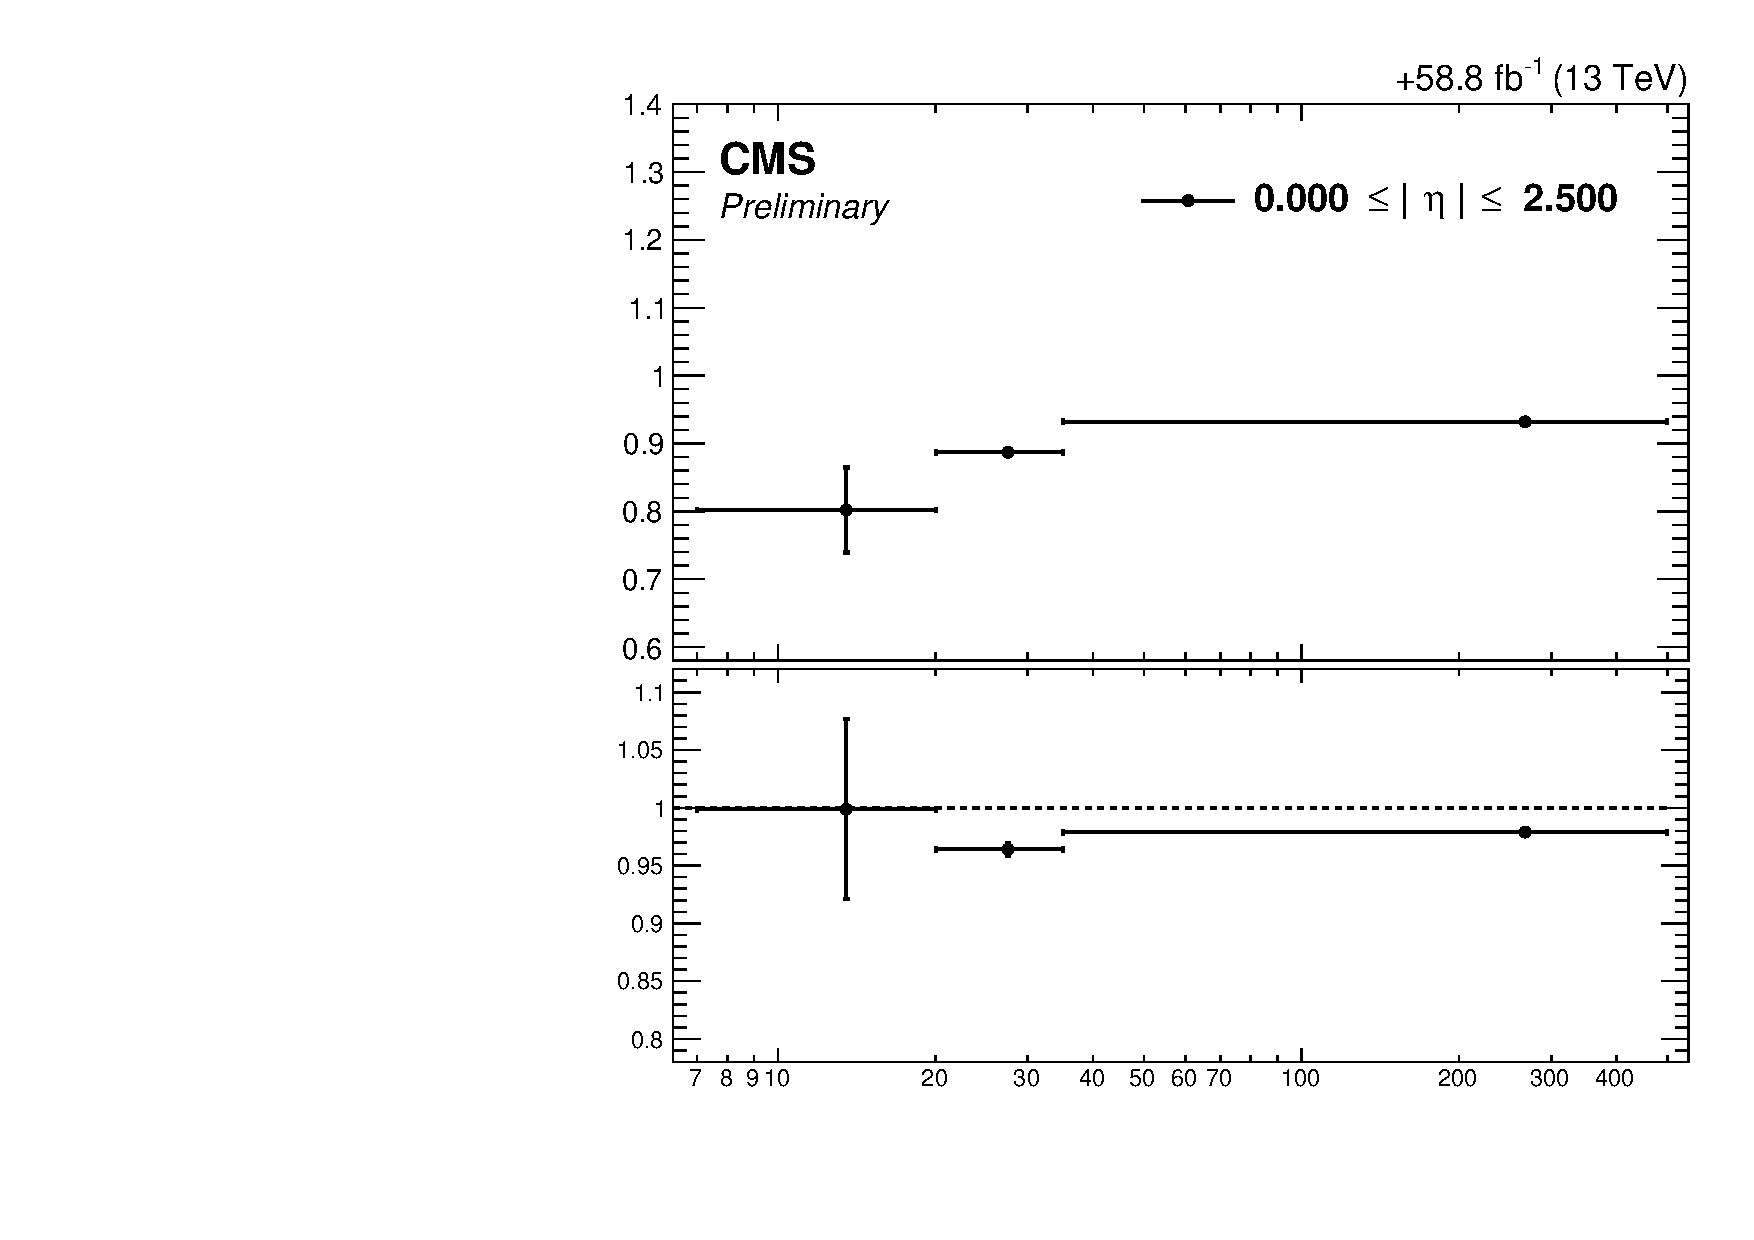
\includegraphics[page=1]{Figures/Electrons/2018_egammaEffitxt_egammaPlotsGAP.pdf}}} \\
    %    \subfigure [] {\resizebox{7.5cm}{!}{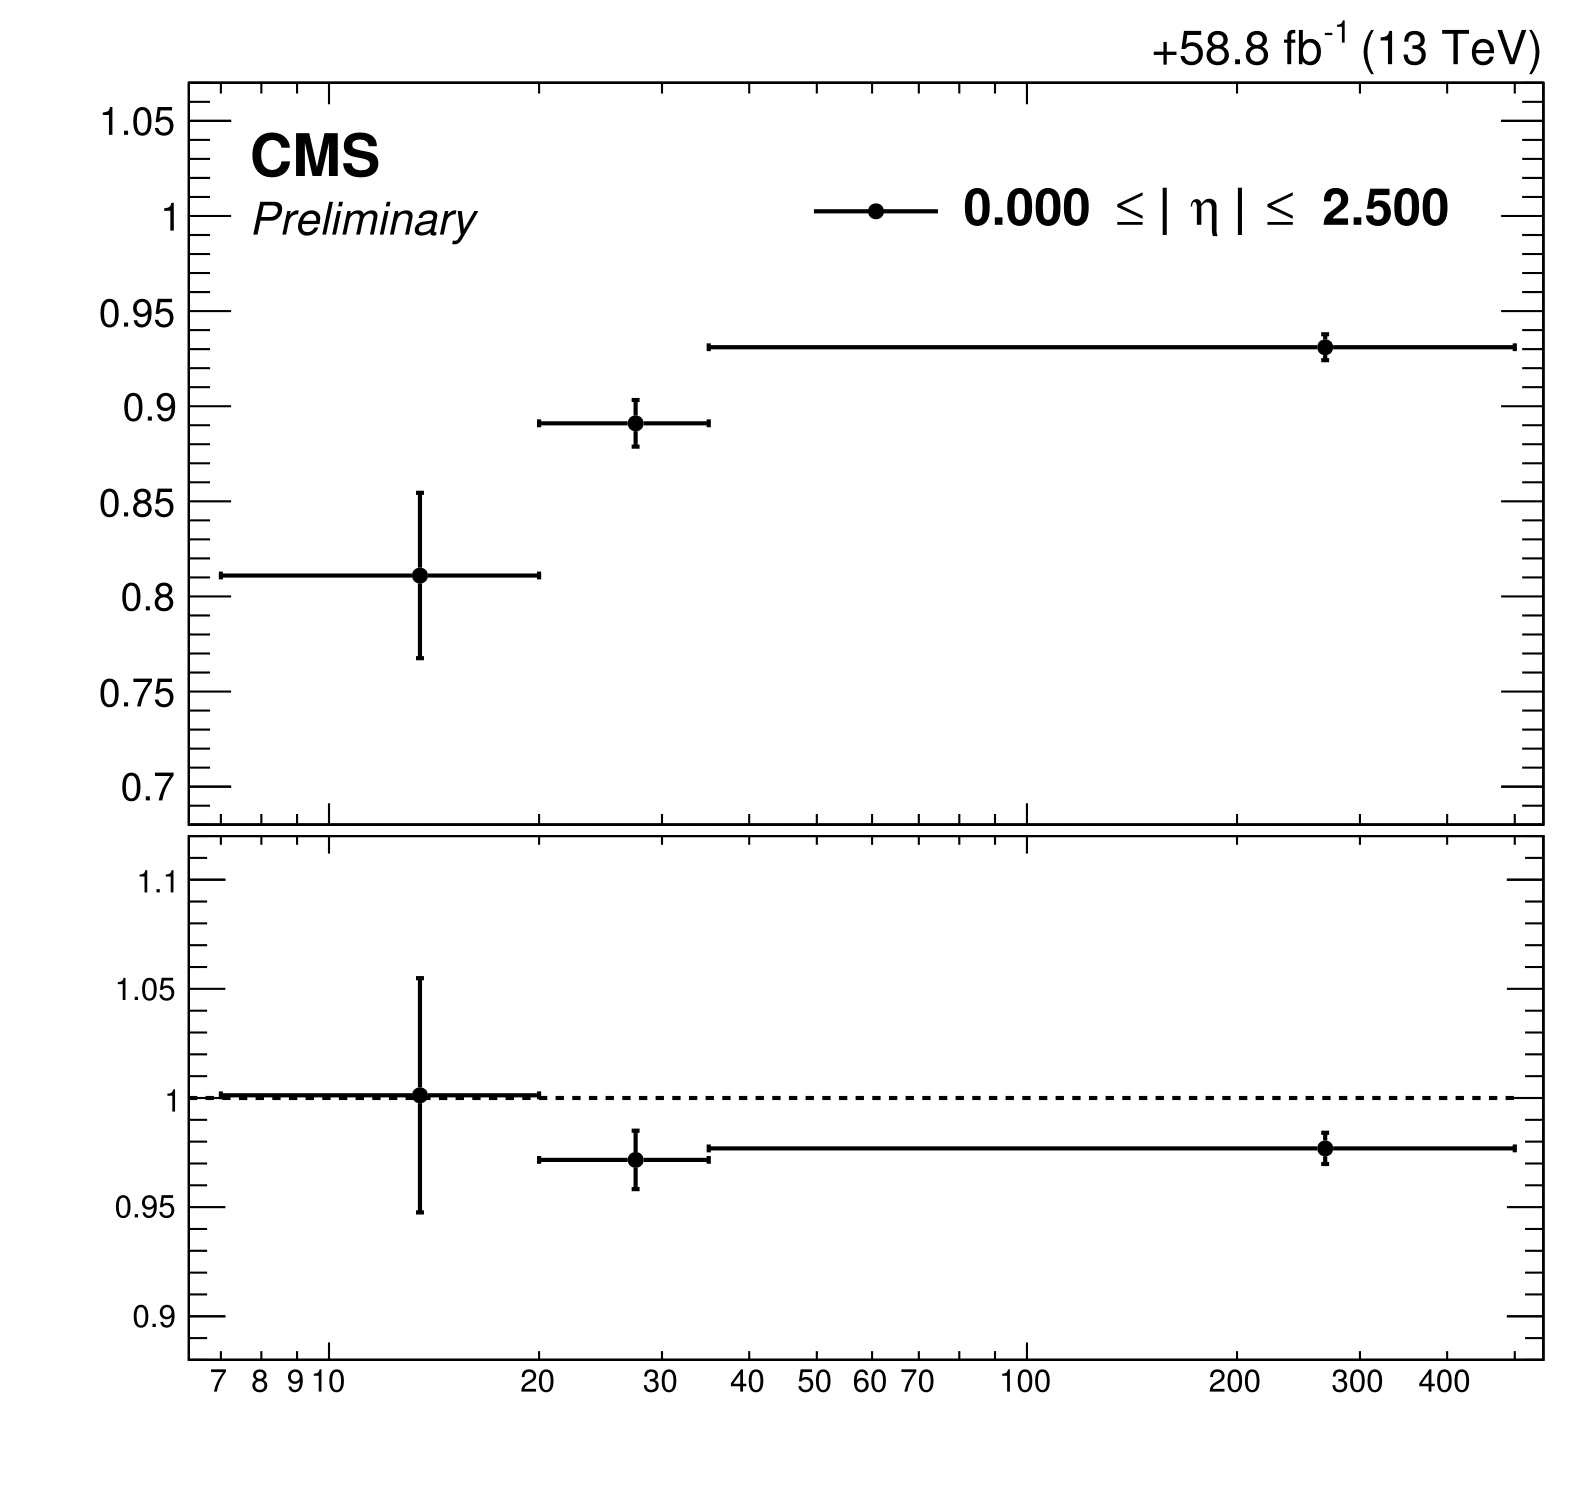
\includegraphics{Figures/Electrons/eleSFvspTgap.png}}}\\
\caption{Electron selection efficiencies vs $p_T$ measured using the Tag-and-Probe technique described in the text, non-gap electrons (left) and gap electrons (right), together with the corresponding data/MC ratio (bottom), for 2018 samples.}
\label{fig:ele_sel_pt_turn_onC}
\end{center}
\end{figure}

\begin{figure}[!htb]
\begin{center}
    \subfigure [] {\resizebox{7.5cm}{!}{\includegraphics[page=2]{Figures/Electrons/2018_egammaEffitxt_egammaPlots.pdf}}}
    \subfigure [] {\resizebox{7.5cm}{!}{\includegraphics[page=2]{Figures/Electrons/2018_egammaEffitxt_egammaPlotsGAP.pdf}}}\\
\caption{Electron selection efficiencies vs $\eta$ measured using the Tag-and-Probe technique described in the text, non-gap electrons (left) and gap electrons (right), together wit the corresponding data/MC ratio at the bottom of each plot, for 2018 samples. Dashed lines is MC, solid lines is DATA.}
\label{fig:ele_sel_eta_turn_onC}
\end{center}
\end{figure}

%\begin{figure}[!htb]
%\begin{center}
%    \subfigure [] {\resizebox{7.5cm}{!}{
\includegraphics{Figures/Placeholder.png}}}
%    \subfigure [] {\resizebox{7.5cm}{!}{
\includegraphics{Figures/Placeholder.png}}}\\
%\caption{2D ($p_T, \eta$) Electron selection Scale Factors measured using the Tag-and-Probe technique described in the text, non-gap electrons (left) and gap electrons (right).}
%\label{fig:ele_sel_scale_factors}
%\end{center}
%\end{figure}


%\paragraph{Systematic uncertainties}\mbox{}\\
%\label{par:Systematic_uncertainties}
%%%%%%%%%%%%%%%%%%%%%%%%%%%%

 The EGM recommendations on the evaluation of Tag-and-Probe uncertainties for efficiency measurements are followed. Specifically, we consider

\begin{itemize}
   \item Variation of the signal shape from a MC shape to an analytic shape (Crystal Ball) fitted to the MC
   \item Variation of the background shape from a CMS-shape to a simple exponential in fits to data
%   \item Variation of the tag selection: tag $p_{T}>$35~GeV and passes MVA-based 8X ID
   \item Using an NLO MC sample for the signal templates
\end{itemize}

The total uncertainty for the measurement of the scale factors is the quadratic sum of the statistical uncertainties returned from the fit and the aforementioned systematic uncertainties.

\clearpage



